\documentclass[svgnames]{beamer}


\mode<presentation>
{
  \usetheme[titleformat=smallcaps,numbering=fraction,progressbar=frametitle]{metropolis}
  \usecolortheme[light,accent=orange]{solarized}
  %\usecolortheme[named=Goldenrod]{structure}
  % or ...

  \setbeamercovered{transparent}
  % or whatever (possibly just delete it)
}


% \usepackage{mathtext}
\usepackage[utf8]{inputenc}
\usepackage[english,russian]{babel}
\usepackage{cmap}
\hypersetup{unicode=true}
\graphicspath{{images/}{slides/images}}


\title[CMTA 04] % (optional, use only with long paper titles)
{Vector space model}

\subtitle
{Computational Methods for Text Analysis} % (optional)

\author%[Author, Another] % (optional, use only with lots of authors)
{Кирилл Александрович Маслинский}
% - Use the \inst{?} command only if the authors have different
%   affiliation.

\institute%[Universities of Somewhere and Elsewhere] % (optional, but mostly needed)
{НИУ ВШЭ Санкт-Петербург}
% - Use the \inst command only if there are several affiliations.
% - Keep it simple, no one is interested in your street address.

\date%[Short Occasion] % (optional)
{04.10.2020 / 04}

\subject{natural language processing, text mining}
% This is only inserted into the PDF information catalog. Can be left
% out. 



% If you have a file called "university-logo-filename.xxx", where xxx
% is a graphic format that can be processed by latex or pdflatex,
% resp., then you can add a logo as follows:

% \pgfdeclareimage[height=0.5cm]{university-logo}{university-logo-filename}
% \logo{\pgfuseimage{university-logo}}

% Delete this, if you do not want the table of contents to pop up at
% the beginning of each subsection:

\newcommand{\plate}[1]{\begingroup\setbeamercolor{background canvas}{bg=Beige}
  % \begin{frame}<beamer>{Outline}
  %   \tableofcontents[sectionstyle=show/hide,subsectionstyle=show/shaded/hide]
  % \end{frame}
  \begin{frame}[plain]
  \vfill
  \centering
  \begin{beamercolorbox}[sep=8pt,center,shadow=true,rounded=true]{title}
    \usebeamerfont{title}#1\par%
  \end{beamercolorbox}
  \vfill
  \end{frame}
  \endgroup
}

% \AtBeginSection[]
% {
%   \begin{frame}<beamer>[plain]{План}
%     \tableofcontents[sectionstyle=shaded,subsectionstyle=hide]
%   \end{frame}
% }

% \AtBeginSubsection[]
% {
%   \begin{frame}<beamer>[plain]{План}
%     \tableofcontents[sectionstyle=shaded,subsectionstyle=show]
%   \end{frame}
% }

\newcommand{\tb}[1]{\colorbox{yellow}{#1}\space}
\newcommand{\Sp}[1]{\colorbox{green}{#1}\space}
\newcommand{\Sn}[1]{\colorbox{red}{#1}\space}


\begin{document}

\begin{frame}
  \titlepage
\end{frame}

\section{Настройка зрения}

\begin{frame}
  \frametitle{Reverse engineering of text}
    \begin{columns}
      \column{.5\textwidth}
      рябчик 2\\
      вкус 1\\
      дичь 1\\
      добывать 1\\
      друг 1\\
      другой 1\\
      каков 1\\
      какой 1\\
      можно 1\\
      москва 1\\
      особенность 1\\
      отличать 1\\
      характерный 1\\
      \column{.5\textwidth}
      \only<2-3>{
        \uncover<3->{а вот} сказать друг каков \uncover<3->{на} вкус рябчик \uncover<3->{быть ли} какой характерный
        особенность отличать \uncover<3->{они от} другой дичь \uncover<3->{и} можно \uncover<3->{ли} рябчик добывать \uncover<3->{в}
        москва
      }
      \only<4>{
        А вот скажите, друзья — каковы на вкус рябчики? Есть ли какие
        характерные особенности, отличающие их от другой дичи? И можно ли
        рябчика добыть в Москве?
      }
    \end{columns}
\end{frame}

\begin{frame}
  \begin{block}{}
    However, I'll argue against the commonly held notion that counting
    words reduces complexity, and I'll suggest instead that semantic
    models embed textual objects in highly complex structures that,
    when constructed using relevant corpora, are extremely sensitive
    to historical context and subtle nuances in meaning.
  \end{block}
  
Michael Gavin \textit{Is there a text in my data? (Part 1): On
Counting Words} // Journal of Cultural Analytics. 09.17.19 
\end{frame}

\section{Векторная модель документа}

\subsection{Bag-of-words: мешок слов}

\begin{frame}
  \frametitle{Модель документа: мешок слов}

  \begin{block}{Для статистического анализа необходимо
      преобразование:}
      Текст $\longrightarrow$ Набор чисел/свойств
  \end{block}

  \begin{itemize}
  \item Каждое слово текста [type] — свойство
  \item Частотность слова — значение свойства
  \end{itemize}
\end{frame}

\begin{frame}[fragile]
  \frametitle{Векторное представление документа}
  \small
  \begin{block}{}
    - Мне, пожалуйста, двойной виски. - Девочка! Это школьная
    столовая! - Ой, извините, я задумалась. Компот, пожалуйста...
  \end{block}
  \footnotesize
\begin{verbatim}
виски    двойной    девочка задумалась   извините 
    1          1          1          1          1 
компот        мне   пожалуйста     столовая     школьн 
     1          1            2            1          1 
это 
  1 
\end{verbatim}
\end{frame}

\subsection{Вектора в многомерном пространстве}

\begin{frame}
  \frametitle{Вектор}
  \begin{columns}
    \column{.5\textwidth}
    \begin{tabular}{ccc}
      \only<2->{ русский & математика & общага \\
        \hline}
      90 & 60 & 90 \\
      \only<3->{
        95 & 65 & 95 \\
        67 & 98 & 100 \\
      }
    \end{tabular}
    \column{.5\textwidth}
\only<4>{
    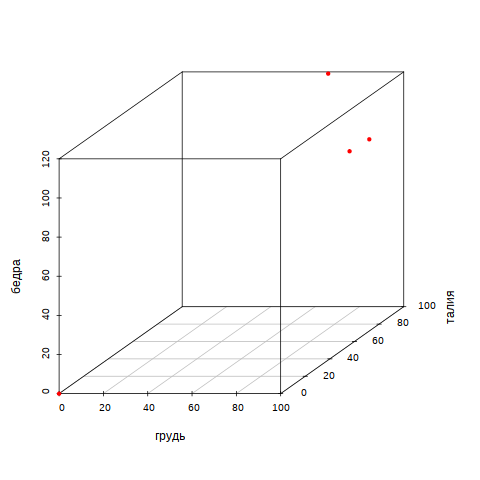
\includegraphics[width=\textwidth]{vectors0}
}
  \end{columns}
\end{frame}

\begin{frame}
  \frametitle{Сходство векторов: евклидово расстояние}
  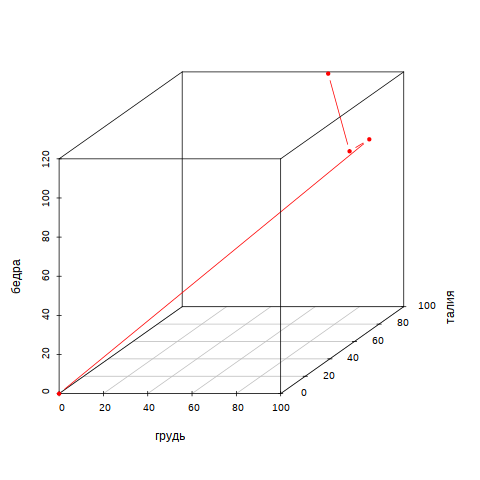
\includegraphics[height=.9\textheight]{vectors1}
\end{frame}

\begin{frame}
  \frametitle{Сходство векторов: косинусная мера}
\only<1>{
  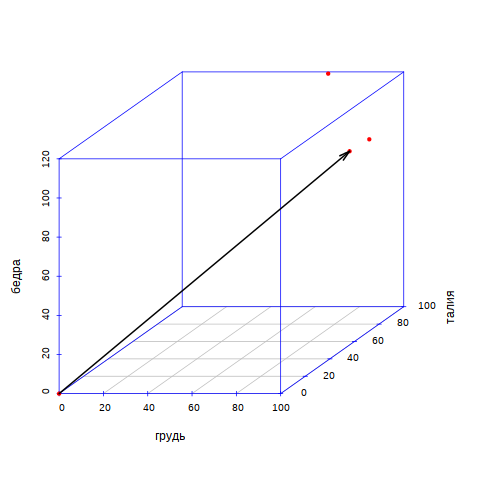
\includegraphics[height=.9\textheight]{vectors2}  
}
\only<2>{
  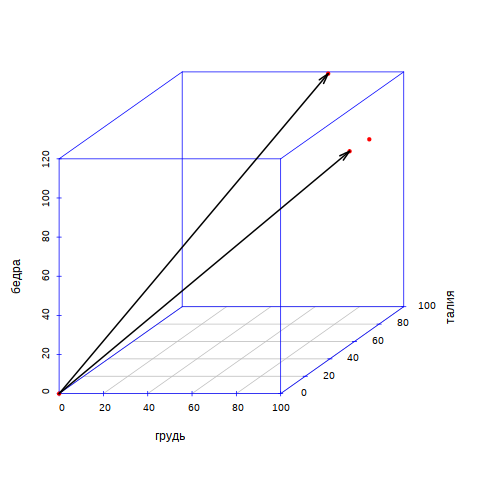
\includegraphics[height=.9\textheight]{vectors3}  
}
\end{frame}

\begin{frame}
  \frametitle{Меры расстояния}
  Сходство документов = близость векторов (в N-мерном пространстве)
  \begin{itemize}
  \item Евклидова мера $L_2(x,y) = \sqrt{\sum_{i=1}^{m}(x_i-y_i)^2}$
  \item $L_1(x,y) = \sum_{i=1}^{m}|x_i-y_i| $   
  \item Косинусная мера $1-\frac{x\cdot y}{|x|\cdot|y|} = 1 -
    \frac{\sum_{i=1}^{n}(A_i\times B_i)}{\sqrt{\sum_{i=1}^{n}(A_i)^2}\sqrt{\sum_{i=1}^{n}(B_i)^2}}$
  \end{itemize}
\end{frame}


\subsection{От частотного списка к матрице}

\begin{frame}[fragile]
  \frametitle{Матрица терминов-документов}
  \framesubtitle{Document-term matrix}
  Термины с наибольшим DF (не менее 15\%)
  \footnotesize
\begin{verbatim}
Docs вовочк дет класс урок учител учительниц школ
   1      2   0     0    1      0          1    0
   2      2   0     0    0      0          1    0
   3      1   1     0    0      0          1    2
   4      3   1     0    1      0          1    0
   5      3   0     0    0      0          1    0
   6      1   0     0    0      0          1    0
\end{verbatim}
\end{frame}

\begin{frame}[standout]
   Матрица частотностей описывает наблюдаемые пересечения двух
   множеств:
   \begin{itemize}
   \item множество допустимых слов (types)
   \item множество допустимых текстовых объектов
   \end{itemize}
\end{frame}

\begin{frame}
  Задавая фиксированный словарь, мы определяем \alert{поле
    возможностей}, в рамках которого могут быть описаны наши
  документы.

  Например, у Шекспира:

  \begin{description}
  \item[ipad] такого слова еще не было (нет смысла его включать)
  \item[theology] мог бы использовать (как некоторые современники), но
    не использовал
  \item[christ] никогда не использовал это слово в комедиях, но зато
    использовал в нескольких исторических пьесах
  \end{description}
\end{frame}

\begin{frame}
  \frametitle{Лексическое пространство $\times$ Пространство документов}
  \begin{itemize}
  \item \textbf{каждый документ} — система из слов, сделанных из
    документов
  \item \textbf{каждое слово} — система из документов, сделанных из
    слов
  \end{itemize}
  \pause
  \begin{block}{Текст в матрице —}
    структурированное множество исторически релевантных связей с
    исторически релевантными контекстами.
  \end{block}
  % Because every document is a system of words made of documents; every
  % word, a system of documents made of words. Rather than say we're
  % representing a document as a series of word frequencies, it's more
  % accurate to say that each text is represented as a structured set of
  % historically relevant relations to historically relevant contexts.
\end{frame}

\section{Анализ корпуса на уровне документов}

\subsection{Лексическая дисперсия}

\begin{frame}
  \frametitle{Распределение лексики по документам}
  \begin{itemize}
  \item Частотность отражает значимость слова в языке/коллекции документов
  \item Но сильно зависит от состава коллекции, ср. частотность слова
    \alert{хоббит}
  \item В дополнение к частотности нужно учитывать \alert{дисперсию} —
    насколько равномерно слово распределено по документам
  \end{itemize}
\end{frame}

\begin{frame}
  \frametitle{IDF: обратная документная частота}
  \begin{equation}
    IDF=\log_2\frac{D}{df}
  \end{equation}
  где 
  \begin{itemize}
  \item[$D$] — количество документов в корпусе
  \item[$df$] — количество документов, содержащих термин ($x$ раз)
  \end{itemize}
\end{frame}

\begin{frame}
  \frametitle{IDF: примеры}
  \begin{tabular}[l]{lccc}
    распределение & D & df & IDF \\
    \hline
    везде & 10000 & 10000 & 0 \\
    часто & 10000 & 1000 & 3,32 \\
    достаточно & 10000 & 100 & 6,64 \\
    несколько & 10000 & 10 & 9,96 \\
    в одном документе & 10000 & 1 & 13,29 \\
  \end{tabular}
\end{frame}


\subsection{Взвешенная частотность: TF-IDF}

\begin{frame}
  \frametitle{Поправка на дисперсию}
  Идея: откорректировать ранжирование в частотном списке в
  соответствии с дисперсией. Задачи:
  \begin{description}
  \item[информационный поиск] понизить ранг слов, распределенных
    равномерно

    Цель — повысить ранг слов, различающих отдельные документы.

  \item[частотные словари] понизить ранг слов, распределенных
    неравномерно

    Цель — понизить ранг слов, получивших неоправданно высокую
    частотность в силу особенностей состава корпуса.
  \end{description}
\end{frame}

\begin{frame}
  \frametitle{TF-IDF}
  Мера, предложенная для информационного поиска: выделение релевантных
  слов документа:
  \begin{equation}
    TF \times IDF = tf\log_2\frac{D}{df}
  \end{equation}
  \begin{itemize}
  \item[$tf$] частота термина (в документе или в коллекции), term frequency
  \item[$df$] число документов, в которых встречается термин, document
    frequency
  \item[$D$] общее число документов в коллекции
  \end{itemize}
\end{frame}

\begin{frame}
  \frametitle{Взвешивание терминов}
  Слова должны \alert{различать} документы:
  \begin{itemize}
  \item не слишком частотные (неинформативны, не позволяют разделять
    различные документы)
  \item не слишком редкие (не позволяют объединять сходные документы)
  \end{itemize}
\end{frame}

\begin{frame}[fragile]
  \frametitle{Нормализация по длине текста}
  Нормализация: разделить каждое значение на количество слов в документе
  \footnotesize
\begin{verbatim}
    Terms
Docs    вовочк       дет класс      урок учител учительниц школ
   1 0.5000000 0.0000000     0 0.2500000      0  0.2500000  0.0
   2 0.6666667 0.0000000     0 0.0000000      0  0.3333333  0.0
   3 0.2000000 0.2000000     0 0.0000000      0  0.2000000  0.4
   4 0.5000000 0.1666667     0 0.1666667      0  0.1666667  0.0
   5 0.7500000 0.0000000     0 0.0000000      0  0.2500000  0.0
   6 0.5000000 0.0000000     0 0.0000000      0  0.5000000  0.0
\end{verbatim}
\end{frame}

\begin{frame}[fragile]
  \frametitle{Взвешивание терминов: TF-IDF}
  Нормализация: вместо частоты слова (TF) его взвешенная частота (IDF)
  \footnotesize
\begin{verbatim}
    Terms
Docs    вовочк       дет класс      урок учител учительниц      школ
   1 0.6897996 0.0000000     0 0.4192463      0  0.4022703 0.0000000
   2 0.9197328 0.0000000     0 0.0000000      0  0.5363604 0.0000000
   3 0.2759198 0.4781918     0 0.0000000      0  0.3218162 0.4736512
   4 0.6897996 0.3984932     0 0.2794975      0  0.2681802 0.0000000
   5 1.0346994 0.0000000     0 0.0000000      0  0.4022703 0.0000000
   6 0.6897996 0.0000000     0 0.0000000      0  0.8045405 0.0000000
\end{verbatim}
\end{frame}

\begin{frame}[fragile]
  \frametitle{Косинусное расстояние}

  \footnotesize
\begin{verbatim}
> dissimilarity(sp, method="cosine")
          1          2         3         4          5
1 0.0000000 0.11461112 0.5542388 0.1226977 0.12552228
2 0.1146111 0.00000000 0.4965362 0.1747931 0.01232358
3 0.5542388 0.49653624 0.0000000 0.3369433 0.53009027
4 0.1226977 0.17479311 0.3369433 0.0000000 0.16449672
5 0.1255223 0.01232358 0.5300903 0.1644967 0.00000000
\end{verbatim}

  \footnotesize
\begin{verbatim}
Docs вовочк дет класс урок учител учительниц школ
   1      2   0     0    1      0          1    0
   2      2   0     0    0      0          1    0
   3      1   1     0    0      0          1    2
   4      3   1     0    1      0          1    0
   5      3   0     0    0      0          1    0
\end{verbatim}

\end{frame}


\end{document}
